\documentclass[border=5pt]{standalone} 
\usepackage{tikz}
\usepackage{tikzsymbols}
\usetikzlibrary{bayesnet}
\usetikzlibrary{arrows}
\usepackage{amsmath}
\begin{document}
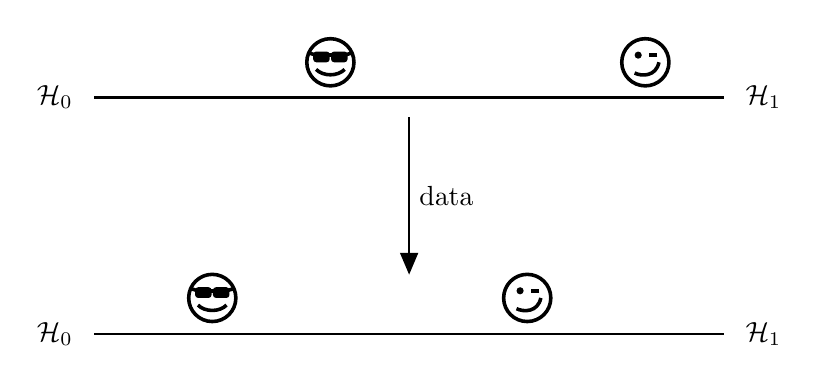
\begin{tikzpicture}
    \node (m1) {$\mathcal{H}_0$};
    \node[right of=m1, xshift=8cm] (m2) {$\mathcal{H}_1$};
    \draw[thick] (0.5,0) -- node[above] {\Cooley[2.5]} ++(6,0) -- node[above] {\Winkey[2.5]} ++(2,0);
      \node[below of=m1, yshift=-2cm] (m1Post) {$\mathcal{H}_0$};
      \node[below of=m2, yshift=-2cm] (m2Post) {$\mathcal{H}_1$};
      \draw[thick] (0.5,-3) -- node[above] {\Cooley[2.5]} ++(3,0) -- node[above] {\Winkey[2.5]} ++(5,0);
      \draw[thick, ->] (4.5,-0.25) -- node[right] {data} ++(0,-2);
    

\end{tikzpicture}
\end{document}
